\section{Hardware}

Die Auswahl der Hardwarekomponenten erfolgte unter Abwägung von Kosten, Kompaktheit und Integrationsfähigkeit.
Ziel war es, eine Systemarchitektur zu definieren, die sämtliche Funktionen des Companion-Bots in einem kompakten, eigenständigen Gerät vereint.
Dabei wurde für jede Teilfunktion, namentlich Recheneinheit, Audioerfassung, visuelle Ausgabe, Audioausgabe und mechanische Ausrichtung, jeweils eine geeignete Komponente identifiziert und deren Integration in das Gesamtsystem geprüft.

\subsection{Ergebnis}

Als zentrale Recheneinheit wurde ein Raspberry Pi gewählt, der aufgrund seiner kompakten Bauform, breiten Softwarekompatibilität und umfangreichen Community-Dokumentation eine geeignete Plattform für ein Embedded-Assistenzsystem darstellt.
Für die Audioerfassung wurde der ReSpeaker 2-Mics Pi HAT eingesetzt, der neben der Sprachaufnahme auch eine richtungsbasierte Schallquellenortung ermöglicht.
Die visuelle Ausgabe erfolgt über ein Waveshare 4-Zoll-IPS-Display, das direkt am Raspberry Pi betrieben wird.
Als Audioausgabe dient ein 5\,W / 8\,$\Omega$-Lautsprecher, der über einen separaten Audioverstärker angesteuert wird.
Die Stromversorgung des Verstärkers erfolgt über einen Arduino Uno.
Für die mechanische Ausrichtung des Kopfteils, das aus Display und Gehäuseoberteil besteht, wird ein Servomotor eingesetzt, der über einen Arduino Nano angesteuert und seriell vom Raspberry Pi kontrolliert wird.
Durch diese Aufteilung der Steuerungsaufgaben auf mehrere Mikrocontroller konnte die Echtzeitfähigkeit der mechanischen und audiovisuellen Komponenten sichergestellt werden, ohne die Hauptrecheneinheit zusätzlich zu belasten.

\begin{figure}[htbp]
    \centering
    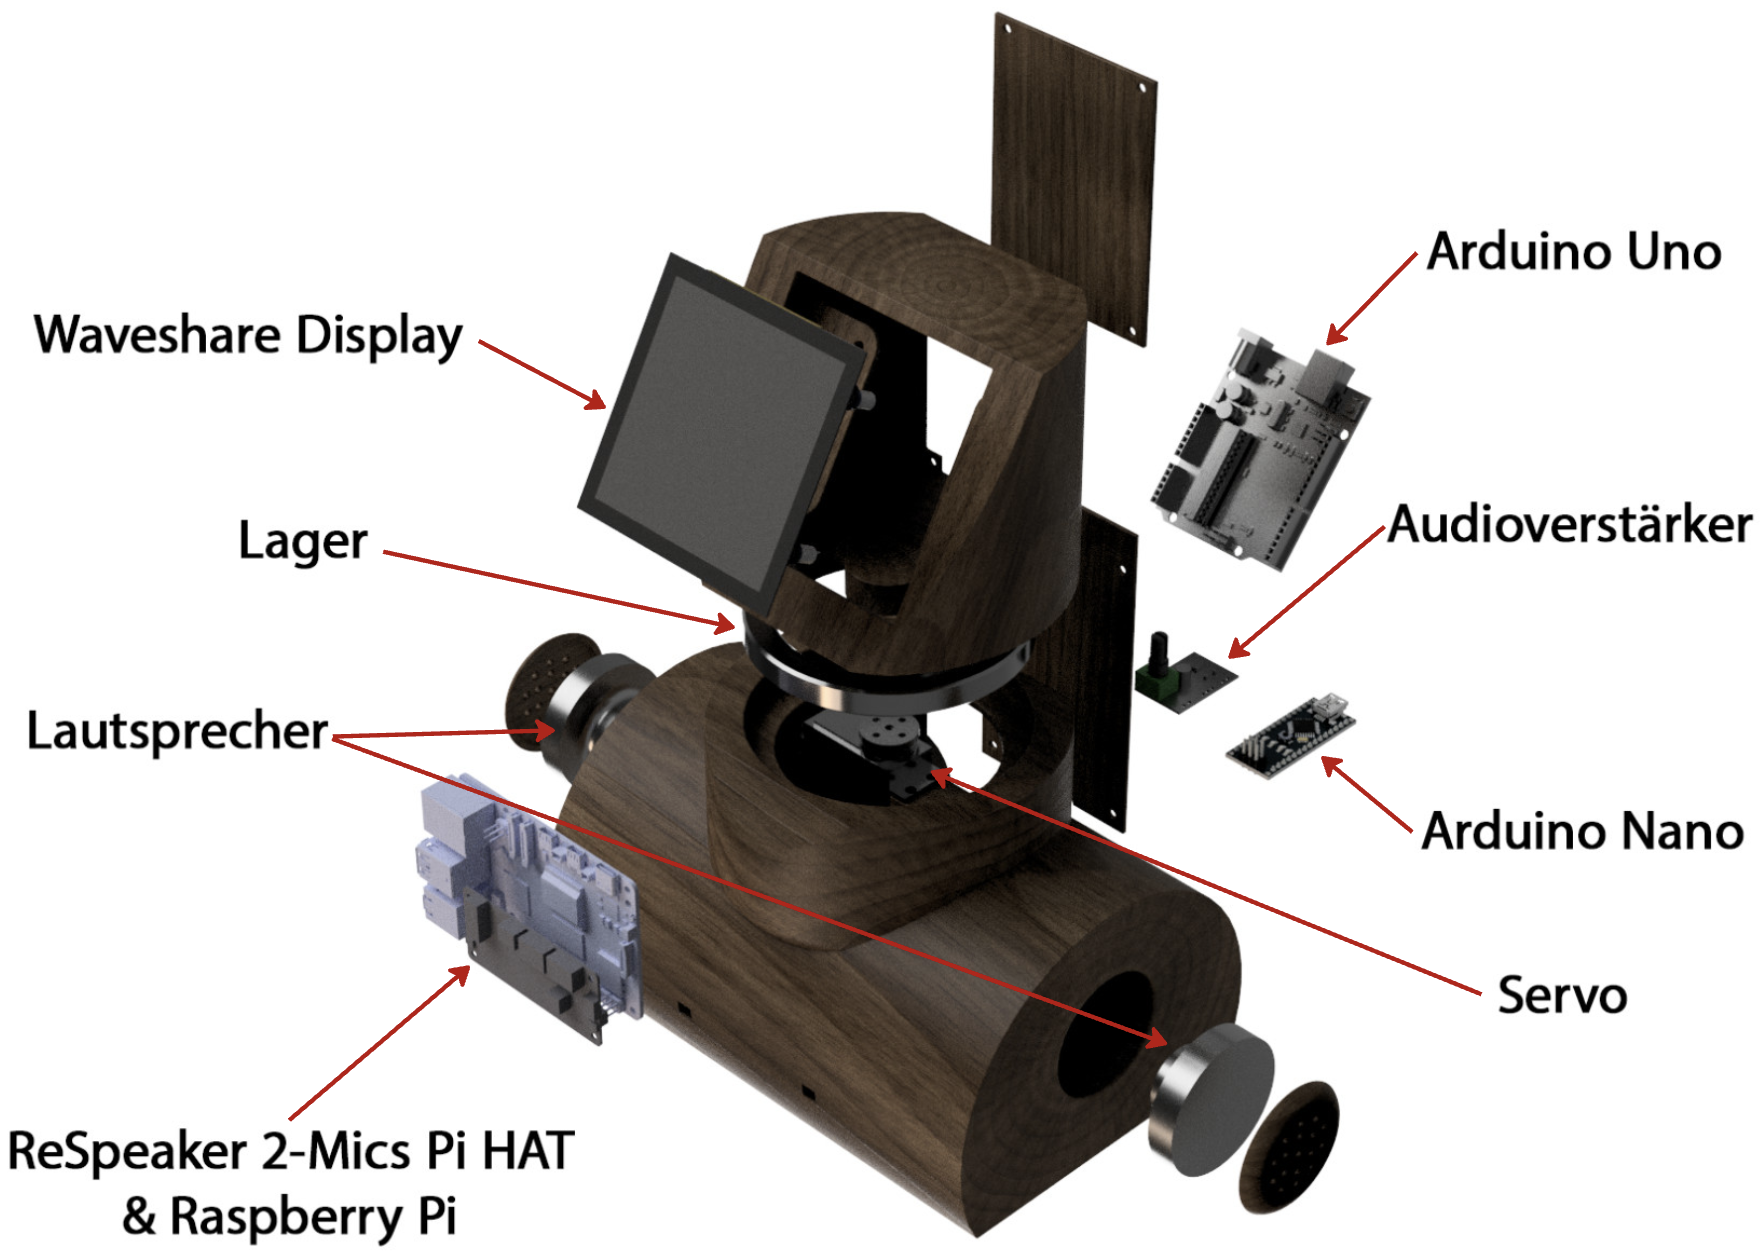
\includegraphics[width=\columnwidth]{grafiken/hardware_explosionsansicht.png}
    \caption{Explosionsansicht des Hardwareaufbaus.}
    \label{fig:hardware_explosion}
\end{figure}

Das Gehäuse wurde als 3D-gedruckter Baumstamm gestaltet und nimmt sämtliche Hardwarekomponenten auf (vgl. Abbildung \ref{fig:hardware_explosion}).
Diese Formgebung unterstreicht den Companion-Charakter von Pablo und schafft eine visuelle Abgrenzung gegenüber rein technischen Geräten.

\begin{table}[htbp]
\centering
\caption{Übersicht der Hardwarekomponenten.}
\label{tab:hardware}
\small
\begin{tabular}{@{}ll@{}}
\toprule
\textbf{Funktion} & \textbf{Komponente} \\
\midrule
Recheneinheit & Raspberry Pi \\
Audioerfassung & ReSpeaker 2-Mics Pi HAT \\
Display & Waveshare 4'' IPS LCD \\
Lautsprecher & 5\,W / 8\,$\Omega$ + Verstärker \\
Energiesteuerung & Arduino Uno \\
Servoansteuerung & Arduino Nano \\
Mechanik & Servomotor \\
Gehäuse & 3D-Druck (Baumstamm) \\
\bottomrule
\end{tabular}
\end{table}


\subsection{Einordnung}

Für die zentrale Recheneinheit wurden verschiedene Plattformen in Betracht gezogen, darunter leistungsfähigere Einplatinencomputer sowie Cloud-basierte Ansätze, bei denen die gesamte Verarbeitung auf einem externen Server erfolgt.
Die Entscheidung fiel auf einen Raspberry Pi, da dieser eine gute Verfügbarkeit, eine breite Community-Unterstützung und eine ausreichende Schnittstellenvielfalt für die Anbindung von Mikrofon, Display, Lautsprecher und Mikrocontrollern bietet.
Obwohl die Rechenleistung im Vergleich zu leistungsstärkeren Alternativen begrenzt ist, reicht sie für die lokale Koordination der einzelnen Systemkomponenten aus.
Zudem eignet sich der Raspberry Pi aufgrund seiner kompakten Bauform besonders gut für den Einsatz in einem Prototyp mit begrenztem Gehäusevolumen.

Alternativ zur Integration eines eigenen Displays wäre eine Ausgabe ausschließlich über Sprache oder über ein externes Gerät wie ein Smartphone möglich gewesen.
Die Entscheidung für ein kompaktes, direkt im Gehäuse verbautes Display wurde getroffen, um Pablo ein lokales visuelles Feedback zu ermöglichen.
Das Display dient der Darstellung des Avatars und der visuellen Begleitung der Sprachinteraktion.
Durch die Integration des Displays in das Gehäuse wird Pablo als eigenständiges, in sich geschlossenes Produkt wahrnehmbar, das keine zusätzlichen externen Geräte für die Nutzung benötigt.